\documentclass[a4paper]{article}
\usepackage{listings}
\usepackage{geometry}
\usepackage[parfill]{parskip}
\usepackage[bottom]{footmisc}

\usepackage[bookmarks=true, bookmarksopen=true]{hyperref}
\usepackage{bookmark}
\usepackage{enumitem}
\usepackage{color}
\definecolor{linkcolour}{rgb}{0,0.2,0.6}
\hypersetup{colorlinks, breaklinks, urlcolor=linkcolour, linkcolor=linkcolour}

\usepackage{amsmath, bm}
\newcommand{\norm}[1]{\left\lVert#1\right\rVert}

\usepackage{csvsimple}

% Font
\usepackage{fontspec}
\setmainfont{GFS Artemisia}

\renewcommand{\figureautorefname}{Σχήμα}
\renewcommand{\tableautorefname}{Πίνακας}

% Images
\usepackage{graphicx}
\graphicspath{{../../}}
\usepackage[font={footnotesize,it}]{caption}
\usepackage[font={footnotesize}]{subcaption}
\renewcommand{\thesubfigure}{\Roman{subfigure}}
\usepackage{float}

% English-Greek use
\usepackage{polyglossia}
\setmainlanguage{greek}
\setotherlanguage{english}

\geometry{
 a4paper,
 total={170mm,257mm},
 left=20mm,
 top=20mm,
}

\title{Υπολογιστική Νοημοσύνη - Στατιστική μάθηση \\ Πρώτη Εργασία}
\author{Κωστινούδης Ευάγγελος \\ΑΕΜ: 112}
\date{\today}

\begin{document}
\maketitle
\pagenumbering{gobble}
\newpage
\pagenumbering{arabic}

\section{Περιγραφή προβλήματος που επιλέχτηκε}

Για την εργασία αυτή επιλέχτηκε το πρόβλημα του διαχωρισμού κλάσεων και τα
δεδομένα προέρχονται από τις βάσεις:

\begin{enumerate}
\item \href{http://yann.lecun.com/exdb/mnist/}{MNIST}
\item \href{https://www.cs.toronto.edu/~kriz/cifar.html}{Cifar-10}
\end{enumerate}


\section{Υλοποίηση}

Για την εκπαίδευση των μοντέλων χρησιμοποιείται τα δεδομένα εκπαίδευσης που
δίνονται από τις δύο βάσεις που χρησιμοποιήθηκαν. Αντίστοιχα χρησιμοποιούνται τα
δεδομένα ελέγχουν για τον έλεγχο των μοντέλων.

\subsection{Επιλογή δειγμάτων}

Από το \autoref{fig:hist} παρατηρείται ότι στο σύνολο εκπαίδευσης κάθε κλάση έχει
τον ίδιο αριθμό δειγμάτων για την βάση Cifar-10, ενώ το αντίστοιχο δεν ισχύει
για την βάση MNIST. Γι᾽ αυτό τον λόγο, υποδειγματοληπτείται το σύνολο
εκπαίδευσης της βάσης MSIST, ούτως ώστε όλες οι κλάσεις να έχουν τον ίδιο αριθμό
δειγμάτων όπως φαίνεται στο \autoref{fig:hist1}. Ο λόγος που επιλέχτηκε η
υποδειγματοληψία είναι ο μεγάλος όγκος δειγμάτων που οδηγεί σε μεγάλο χρονικό
διάστημα εκτέλεσης των πειραμάτων.

\begin{figure}[H]
    \centering

    \begin{subfigure}[t]{0.48\linewidth}
    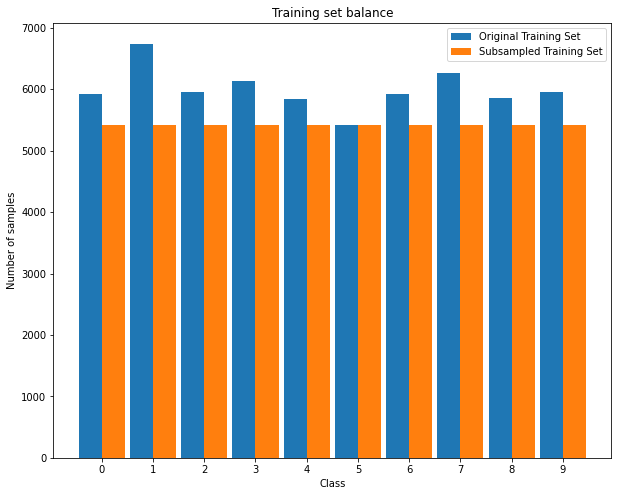
\includegraphics[width=\linewidth]{figures/mnist/training_freq.png}
    \caption{Ιστόγραμμα κλάσεων πριν και μετά την υποδειγματοληψία για τη βάση
    MNIST}
    \label{fig:hist1}
    \end{subfigure}
    \begin{subfigure}[t]{0.48\linewidth}
    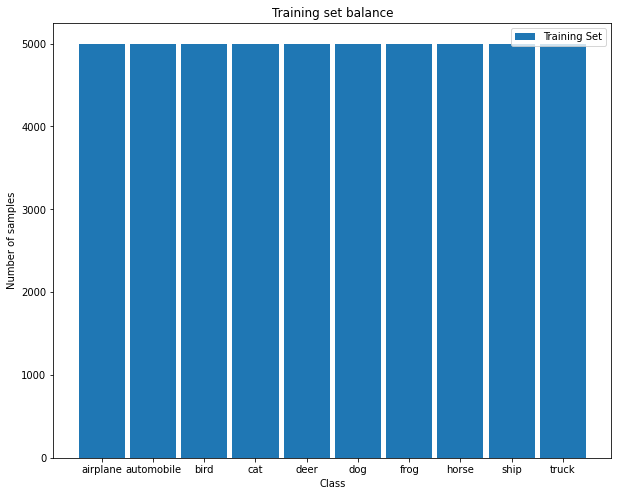
\includegraphics[width=\linewidth]{figures/cifar/training_freq.png}
    \caption{Ιστόγραμμα κλάσεων για τη βάση Cifar-10}
    \end{subfigure}

    \caption{Ιστογράμματα κλάσεων για τις βάσεις δεδομένων}
    \label{fig:hist}
\end{figure}

\subsection{Προεπεξεργασία δεδομένων}

Σε αυτό το στάδιο εφαρμόζεται η παρακάτω διαδικασία και για τις δύο βάσεις:

\begin{enumerate}
    \item Μετασχηματισμός των δεδομένων στο διάστημα $[0,1]$ για κάθε
        χαρακτηριστικό των δεδομένων.
    \item Εφαρμογή της μεθόδου PCA, κρατώντας τουλάχιστον 90\% της πληροφορίας.
    \item Μετασχηματισμός των δεδομένων στο διάστημα $[0,1]$ για κάθε
        χαρακτηριστικό των δεδομένων ξανά.
\end{enumerate}

Ο πρώτος μετασχηματισμός είναι περιττός αφού τα δεδομένα είναι 8-bit εικόνες,
που σημαίνει ότι όλα τα χαρακτηριστικά βρίσκονται στο ίδιο διάστημα ($[0-255]$).

\subsection{Επιλογή παραμέτρων}

Τα μοντέλα που επιλέχτηκαν είναι:

\begin{enumerate}
    \item Γραμμικό SVM
    \item SVM με πολυωνυμικό πυρήνα
    \item SVM με RBF πυρήνα
    \item SVM με σιγμοειδή πυρήνα
\end{enumerate}

Και τα αποτελέσματα τους συγκρίθηκαν και με τις μεθόδους πλησιέστερων γειτόνων
(Nearest Neighbors) και πλησιέστερου κέντρου κλάσης (Nearest Class Centroid).

Για κάθε μοντέλο υλοποιήθηκε η μέθοδος αναζήτησης πλέγματος (grid search) για
την εύρεση των καλύτερων παραμέτρων εκτός του μοντέλου πλησιέστερου κέντρου
κλάσης, όπου χρησιμοποιήθηκε η ευκλείδεια απόσταση.

Συγκεκριμένα για τη βάση MNIST χρησιμοποιήθηκε 3-fold cross validation για τις
παραμέτρους:

\begin{enumerate}
    \item Γραμμικό SVM: $C: (0.1, 1, 10)$
    \item SVM με πολυωνυμικό πυρήνα: $C: (0.1, 1, 10), d: (2, 3, 4), \gamma:
        (0.1, 1, 10)$
    \item SVM με RBF πυρήνα: $C: (1, 10, 50), \gamma: (0.01, 0.1, 1, 10, 100)$
    \item SVM με σιγμοειδή πυρήνα: $C: (10, 100, 1000, 10000), \gamma: (0.0001,
        0.001, 0.01, 0.1)$
\end{enumerate}

Για τη βάση Cifar-10 χρησιμοποιήθηκε 2-fold cross validation για τις
παραμέτρους:

\begin{enumerate}
    \item Γραμμικό SVM: $C: (0.1, 1, 10)$
    \item SVM με πολυωνυμικό πυρήνα: $C: (0.1, 1, 10), d: (2, 3), \gamma:
        (0.1, 1)$
    \item SVM με RBF πυρήνα: $C: (1, 10, 50), \gamma: (0.1, 1, 10)$
    \item SVM με σιγμοειδή πυρήνα: $C: (10, 100, 1000), \gamma: (0.0001, 0.001,
        0.01)$
\end{enumerate}

Όπου $C$ είναι η παράμετρος του σφάλματος από της εξίσωση:

\begin{equation*}
\begin{split}
    \min_{\bm{w},b,\bm{\xi}} & \frac{1}{2} \bm{w}^T\bm{w} + C \sum_{i} \xi_{i} \\
    \text{subject to } & y_i (\bm{w^T} \phi (\bm{x}_i) + b) \ge 1 - \xi_i \\
     & \xi_i \ge 0
\end{split}
\end{equation*}

Επίσης οι υπόλοιπες παράμετροι για κάθε πυρήνα είναι:

\begin{enumerate}
    \item SVM με πολυωνυμικό πυρήνα: $K(\bm{x}_i,\bm{x}_j) = (\gamma \bm{x}_i^T
        \bm{x}_j)^d$
    \item SVM με RBF πυρήνα: $K(\bm{x}_i,\bm{x}_j) = exp(-\gamma
        \norm{\bm{x}_i - \bm{x}_j}^2)$
    \item SVM με σιγμοειδή πυρήνα: $K(\bm{x}_i,\bm{x}_j) = tanh(\gamma
        \bm{x}_i^T \bm{x}_j)$
\end{enumerate}

Για το μοντέλο πλησιέστερων γειτόνων και για τις δύο βάσεις χρησιμοποιήθηκε
3-fold cross validation για τις παραμέτρους $n\_neighbors: (1, 3, 5, 10, 30,
100, 200), weights: (uniform, distance)$ όπου $n\_neighbors$ ο αριθμός των
γειτόνων και $weights$ η χρήση βαρών ($distance$ υπολογισμός βαρών μέσω της
ευκλείδειας απόστασης και $uniform$ ομοιόμορφα βάρη).

Η μετρική για την επιλογή των παραμέτρων είναι το macro F1-score δηλαδή ο μέσος
όρος των F1-scores για κάθε κλάση.

Ο λόγος που επιλέχτηκαν παραπάνω παράμετροι για τη βάση MNIST αλλά και
περισσότερες τιμές στο cross validation είναι ο χρόνος εκτέλεσης των πειραμάτων.
Με τις παραμέτρους αυτές ο χρόνος εκτέλεσης των πειραμάτων για τις δύο βάσεις
είναι παρόμοιος, όπως θα αναφερθεί και παρακάτω.

\section{Αποτελέσματα}

Τα πειράματα εκτελέστηκαν στο περιβάλλον του
\href{https://colab.research.google.com/}{Google Colab}.

\subsection{Επιλογή παραμέτρων}

\subsubsection{Γραμμικό SVM}

Από το \autoref{fig:cv_linear} παρατηρείται ότι για το μοντέλο του γραμμικού SVM
η καλύτερη παράμετρος του $C$ για τη βάση MNIST είναι {\bf10} ενώ για την βάση
Cifar-10 είναι {\bf1}.

\begin{figure}[H]
    \centering

    \begin{subfigure}[t]{0.45\linewidth}
    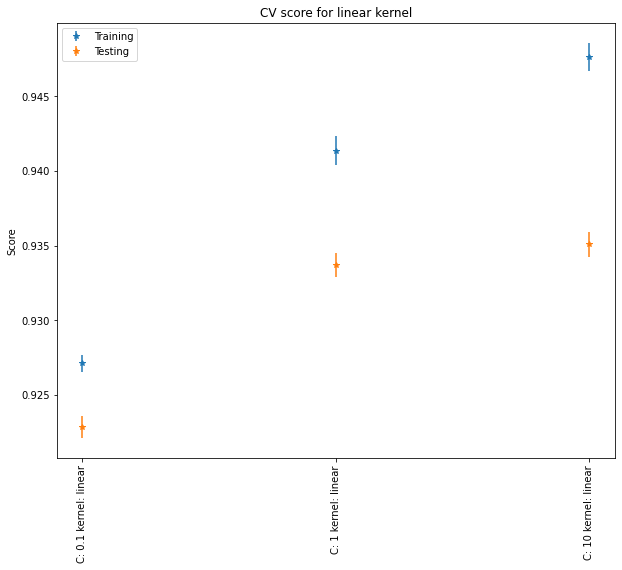
\includegraphics[width=\linewidth]{figures/mnist/cv_results_linear.png}
    \caption{MNIST}
    \end{subfigure}
    \begin{subfigure}[t]{0.45\linewidth}
    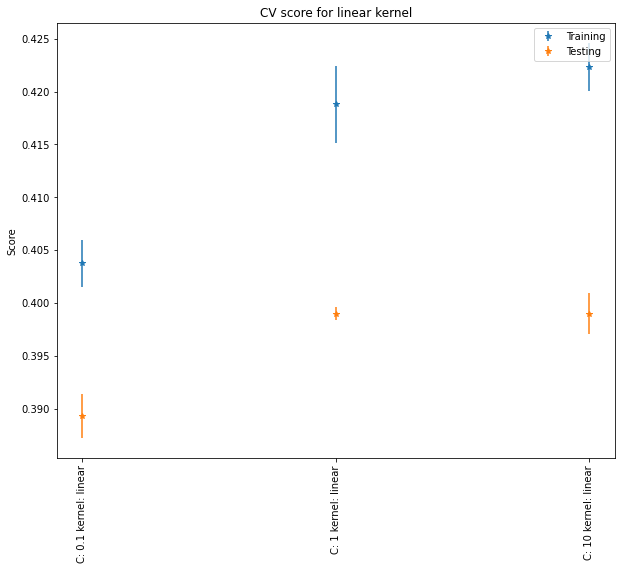
\includegraphics[width=\linewidth]{figures/cifar/cv_results_linear.png}
    \caption{Cifar-10}
    \end{subfigure}

    \caption{Αποτελέσματα αναζήτησης πλέγματος για το γραμμικό SVM.}
    \label{fig:cv_linear}
\end{figure}

\subsubsection{SVM με πολυωνυμικό πυρήνα}

Από το \autoref{fig:cv_poly} παρατηρείται ότι για το μοντέλο του SVM με
πολυωνυμικό πυρήνα οι καλύτερες παράμετροι για κάθε βάση δίνονται στο
\autoref{tab:best_poly}.

\begin{table}[h]
\centering
\begin{tabular}{|c|c|c|}
\hline
         & MNIST & Cifar-10 \\ \hline
$C$      & 10    & 1        \\ \hline
$\gamma$ & 0.1   & 1        \\ \hline
$d$      & 4     & 2        \\ \hline
\end{tabular}
\caption{Καλύτεροι παράμετροι SVM με πολυωνυμικό πυρήνα}
\label{tab:best_poly}
\end{table}

\begin{figure}[H]
    \centering

    \begin{subfigure}[t]{0.45\linewidth}
    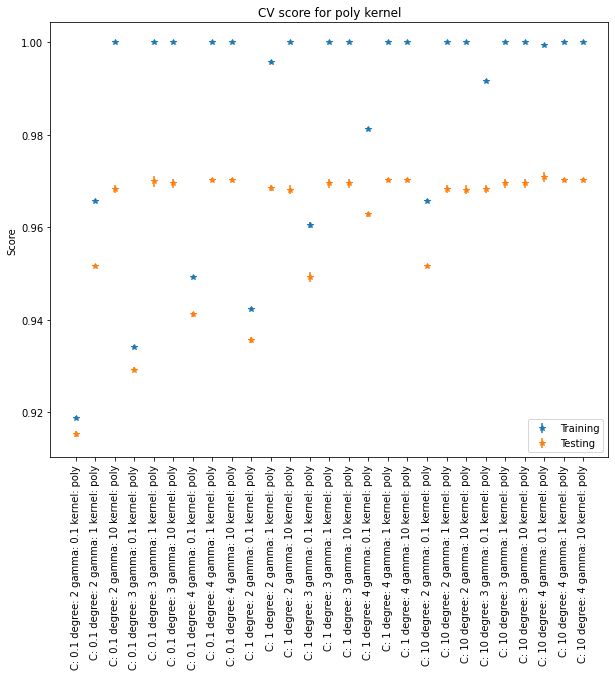
\includegraphics[width=\linewidth]{figures/mnist/cv_results_poly.png}
    \caption{MNIST}
    \end{subfigure}
    \begin{subfigure}[t]{0.45\linewidth}
    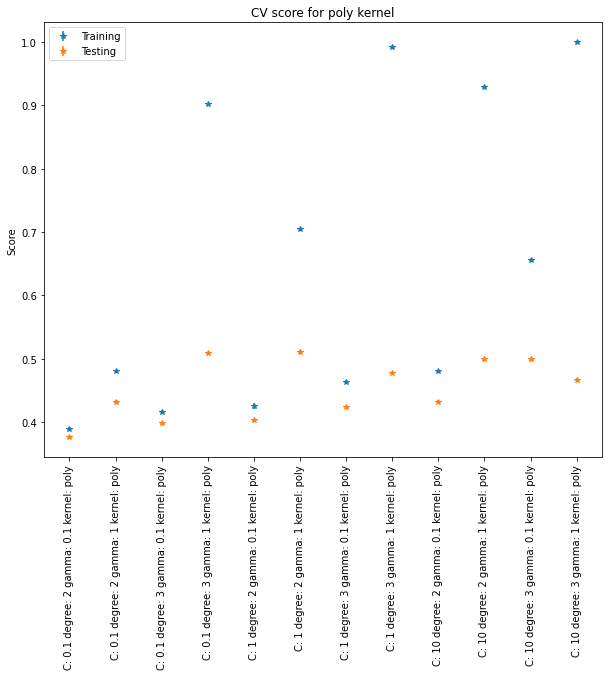
\includegraphics[width=\linewidth]{figures/cifar/cv_results_poly.png}
    \caption{Cifar-10}
    \end{subfigure}

    \caption{Αποτελέσματα αναζήτησης πλέγματος για το SVM με πολυωνυμικό
    πυρήνα.}
    \label{fig:cv_poly}
\end{figure}


\subsubsection{SVM με RBF πυρήνα}

Από το \autoref{fig:cv_rbf} παρατηρείται ότι για το μοντέλο του SVM με RBF
πυρήνα οι καλύτερες παράμετροι για κάθε βάση δίνονται στο
\autoref{tab:best_rbf}.

\begin{table}[h]
\centering
\begin{tabular}{|c|c|c|}
\hline
         & MNIST & Cifar-10 \\ \hline
$C$      & 10    & 10       \\ \hline
$\gamma$ & 1     & 1        \\ \hline
\end{tabular}
\caption{Καλύτεροι παράμετροι SVM με RBF πυρήνα}
\label{tab:best_rbf}
\end{table}

\begin{figure}[H]
    \centering

    \begin{subfigure}[t]{0.45\linewidth}
    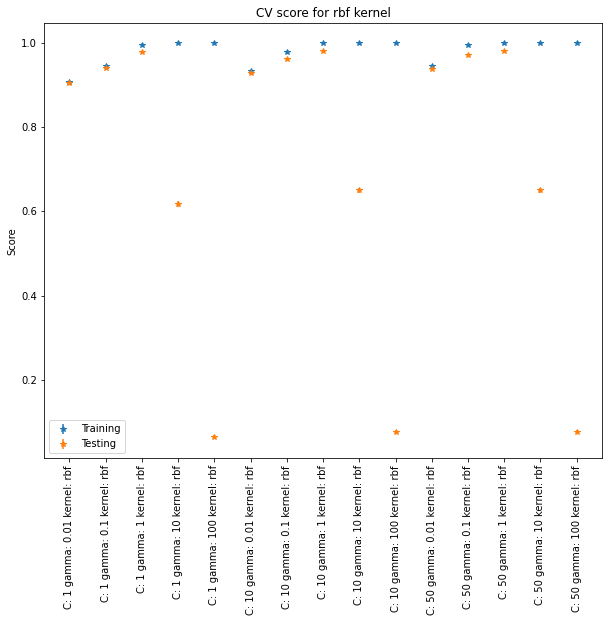
\includegraphics[width=\linewidth]{figures/mnist/cv_results_rbf.png}
    \caption{MNIST}
    \end{subfigure}
    \begin{subfigure}[t]{0.45\linewidth}
    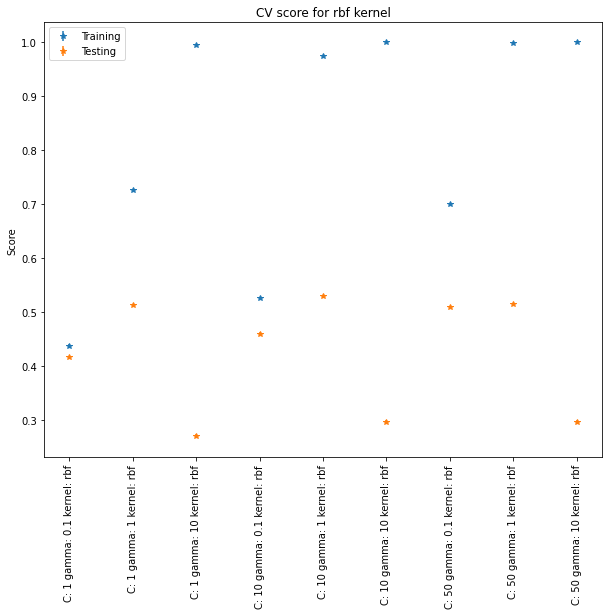
\includegraphics[width=\linewidth]{figures/cifar/cv_results_rbf.png}
    \caption{Cifar-10}
    \end{subfigure}

    \caption{Αποτελέσματα αναζήτησης πλέγματος για το SVM με RBF πυρήνα.}
    \label{fig:cv_rbf}
\end{figure}


\subsubsection{SVM με σιγμοειδή πυρήνα}

Από το \autoref{fig:cv_sigmoid} παρατηρείται ότι για το μοντέλο του SVM με
σιγμοειδή πυρήνα οι καλύτερες παράμετροι για κάθε βάση δίνονται στο
\autoref{tab:best_sigmoid}.

\begin{table}[h]
\centering
\begin{tabular}{|c|c|c|}
\hline
         & MNIST & Cifar-10 \\ \hline
$C$      & 10000 & 10000    \\ \hline
$\gamma$ & 0.001 & 0.001    \\ \hline
\end{tabular}
\caption{Καλύτεροι παράμετροι SVM με σιγμοειδή πυρήνα}
\label{tab:best_sigmoid}
\end{table}

\begin{figure}[H]
    \centering

    \begin{subfigure}[t]{0.45\linewidth}
    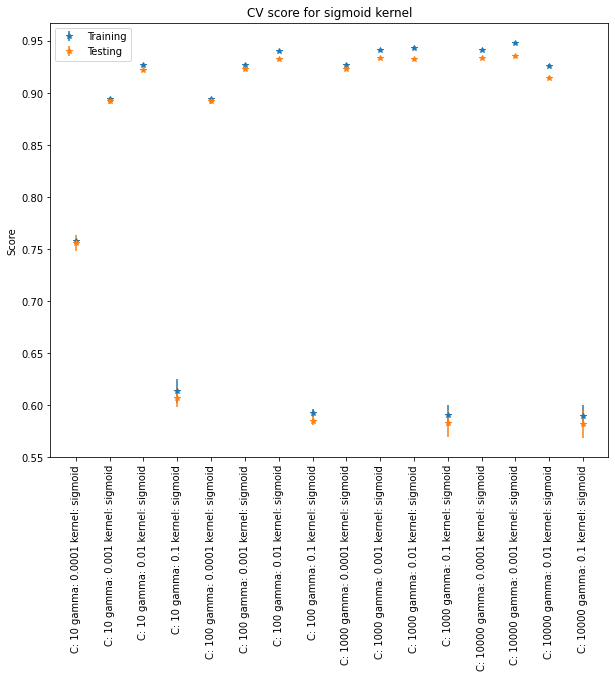
\includegraphics[width=\linewidth]{figures/mnist/cv_results_sigmoid.png}
    \caption{MNIST}
    \end{subfigure}
    \begin{subfigure}[t]{0.45\linewidth}
    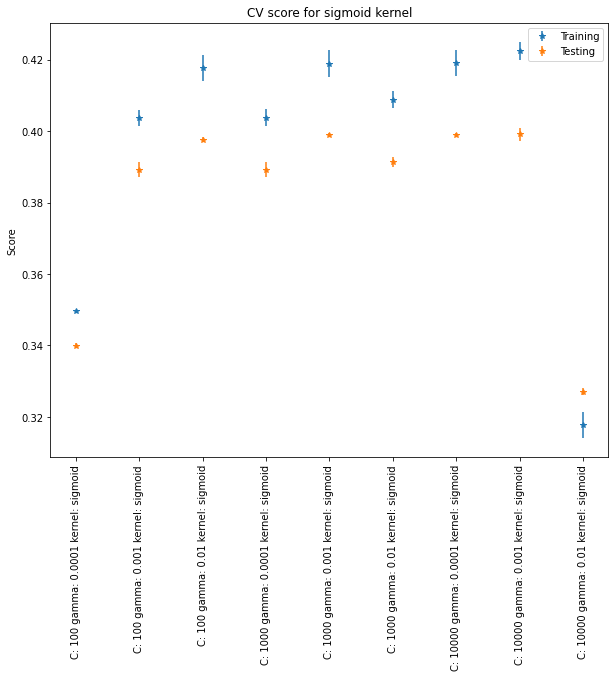
\includegraphics[width=\linewidth]{figures/cifar/cv_results_sigmoid.png}
    \caption{Cifar-10}
    \end{subfigure}

    \caption{Αποτελέσματα αναζήτησης πλέγματος για το SVM με σιγμοειδή πυρήνα.}
    \label{fig:cv_sigmoid}
\end{figure}

\subsubsection{πλησιέστερων γειτόνων}

Από το \autoref{fig:cv_knn} παρατηρείται ότι για το μοντέλο των πλησιέστερων
γειτόνων οι καλύτερες παράμετροι για κάθε βάση δίνονται στο
\autoref{tab:best_knn}.

\begin{table}[h]
\centering
\begin{tabular}{|c|c|c|}
\hline
               & MNIST    & Cifar-10 \\ \hline
$n\_neighbors$ & 3        & 1        \\ \hline
$weights$      & distance & uniform  \\ \hline
\end{tabular}
\caption{Καλύτεροι παράμετροι πλησιέστερων γειτόνων}
\label{tab:best_knn}
\end{table}

\begin{figure}[H]
    \centering

    \begin{subfigure}[t]{0.45\linewidth}
    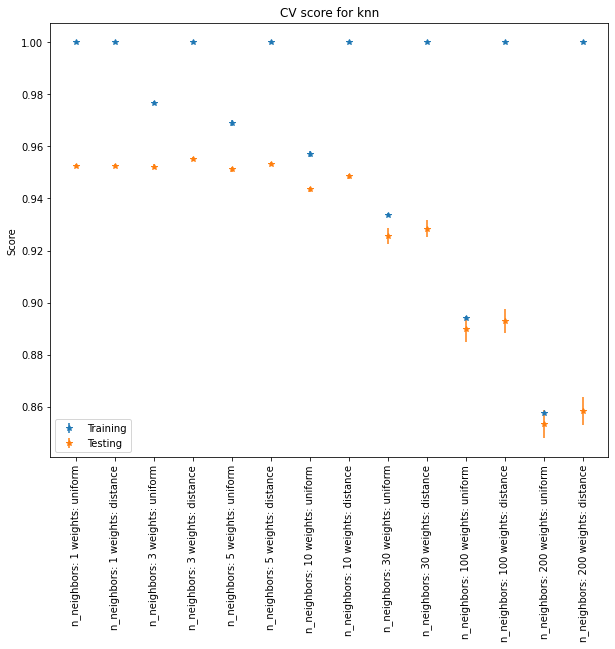
\includegraphics[width=\linewidth]{figures/mnist/cv_results_knn.png}
    \caption{MNIST}
    \end{subfigure}
    \begin{subfigure}[t]{0.45\linewidth}
    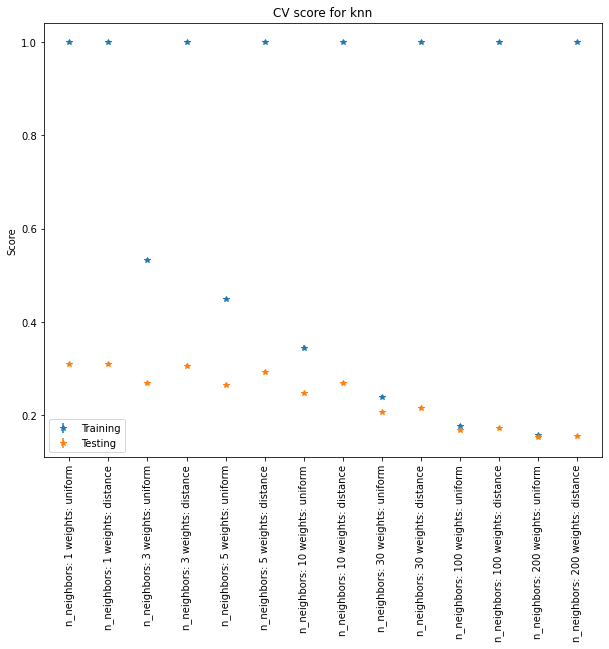
\includegraphics[width=\linewidth]{figures/cifar/cv_results_knn.png}
    \caption{Cifar-10}
    \end{subfigure}

    \caption{Αποτελέσματα αναζήτησης πλέγματος για το μοντέλο πλησιέστερων
    γειτόνων.}
    \label{fig:cv_knn}
\end{figure}

\subsection{Απόδοση μοντέλων}

Αφού έχουν επιλεγεί οι καλύτερες παράμετροι για κάθε μοντέλο και έχουν
εκπαιδευτεί όλα τα μοντέλα στο σύνολο εκπαίδευσης για κάθε βάση, θα συγκριθεί η
απόδοση τους.

\subsubsection{MNIST}

Στο \autoref{fig:mnist_metrics} και στους \autoref{tab:mnist_train} και
\autoref{tab:mnist_test} φαίνονται τα αποτελέσματα των μετρικών για όλα τα
μοντέλα στο σύνολο εκπαίδευσης και ελέγχου για τις καλύτερες παραμέτρους στη
βάση MNIST.

Το μοντέλο του SVM με RBF πυρήνα έχει το καλύτερο αποτέλεσμα για όλες τις
μετρικές στο σύνολο ελέγχου. Το μοντέλο των πλησιέστερων γειτόνων έχει καλύτερα
αποτελέσματα από αυτά των SVM με γραμμικό και σιγμοειδή πυρήνα και το μοντέλο
του πλησιέστερου κέντρου κλάσης έχει τα χειρότερα αποτελέσματα.

Από το \autoref{fig:mnist_training_times} και τον \autoref{tab:mnist_train}
φαίνεται ο χρόνος εκπαίδευσης των μοντέλων. Το μοντέλο του SVM με RBF πυρήνα που
έχει τα καλύτερα αποτελέσματα έχει το μεγαλύτερο χρόνο εκπαίδευσης. Επίσης, τα
μοντέλα των πλησιέστερων γειτόνων και του πλησιέστερου κέντρου κλάσης έχουν πολύ
πιο μικρό χρόνο εκπαίδευσης σε σχέση με τα μοντέλα SVM.

\begin{table}[h]
\begin{tabular}{|l|c|c|c|c|c|}
\hline
\textbf{Model}                                                                        & \textbf{Accuracy} & \textbf{Precision} & \textbf{Recall} & \textbf{F1} & \textbf{Training Time (seconds)} \\ \hline
\begin{tabular}[c]{@{}l@{}}C: 10\\ kernel: linear\end{tabular}                        & 0,9461            & 0,946              & 0,9461          & 0,946       & 57,5676                          \\ \hline
\begin{tabular}[c]{@{}l@{}}C: 10\\ degree: 4\\ gamma: 0.1\\ kernel: poly\end{tabular} & 0,9993            & 0,9993             & 0,9993          & 0,9993      & 54,2103                          \\ \hline
\begin{tabular}[c]{@{}l@{}}C: 10\\ gamma: 1\\ kernel: rbf\end{tabular}                & 1                 & 1                  & 1               & 1           & 125,2382                         \\ \hline
\begin{tabular}[c]{@{}l@{}}C: 10000\\ gamma: 0.001\\ kernel: sigmoid\end{tabular}     & 0,946             & 0,9459             & 0,946           & 0,9459      & 63,1962                          \\ \hline
\begin{tabular}[c]{@{}l@{}}n\_neighbors: 3\\ weights: distance\end{tabular}           & 1                 & 1                  & 1               & 1           & 0,0161                           \\ \hline
Nearest Centroid                                                                      & 0,8495            & 0,852              & 0,8495          & 0,8496      & 0,0508                           \\ \hline
\end{tabular}
\centering
\caption{Μετρικές αποτελεσμάτων στο σύνολο εκπαίδευσης και χρόνος εκπαίδευσης
    για τη βάση MNIST.}
\label{tab:mnist_train}
\end{table}

\begin{table}[h]
\begin{tabular}{|l|c|c|c|c|c|}
\hline
\textbf{Model}                                                                        & \textbf{Accuracy} & \textbf{Precision} & \textbf{Recall} & \textbf{F1} \\ \hline
\begin{tabular}[c]{@{}l@{}}C: 10\\ kernel: linear\end{tabular}                        & 0,9436            & 0,9429             & 0,9428          & 0,9427      \\ \hline
\begin{tabular}[c]{@{}l@{}}C: 10\\ degree: 4\\ gamma: 0.1\\ kernel: poly\end{tabular} & 0,9777            & 0,9776             & 0,9775          & 0,9776      \\ \hline
\begin{tabular}[c]{@{}l@{}}C: 10\\ gamma: 1\\ kernel: rbf\end{tabular}                & 0,9841            & 0,984              & 0,9841          & 0,984       \\ \hline
\begin{tabular}[c]{@{}l@{}}C: 10000\\ gamma: 0.001\\ kernel: sigmoid\end{tabular}     & 0,9437            & 0,943              & 0,9429          & 0,9428      \\ \hline
\begin{tabular}[c]{@{}l@{}}n\_neighbors: 3\\ weights: distance\end{tabular}           & 0,9579            & 0,9584             & 0,9575          & 0,9576      \\ \hline
Nearest Centroid                                                                      & 0,8606            & 0,8614             & 0,859           & 0,8594      \\ \hline
\end{tabular}
\centering
\caption{Μετρικές αποτελεσμάτων στο σύνολο ελέγχο για τη βάση MNIST.}
\label{tab:mnist_test}
\end{table}

\begin{figure}[H]
    \centering
    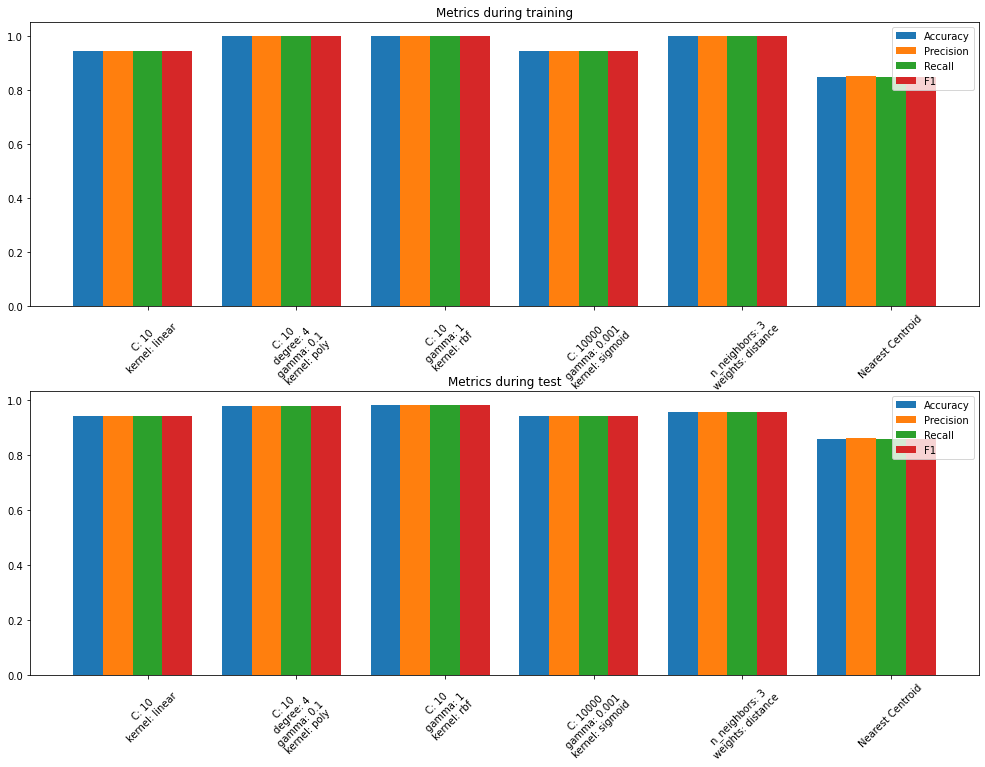
\includegraphics[width=\linewidth]{figures/mnist/all_metrics.png}
    \caption{Μετρικές για τη βάση MNIST}
    \label{fig:mnist_metrics}
\end{figure}

\begin{figure}[H]
    \centering
    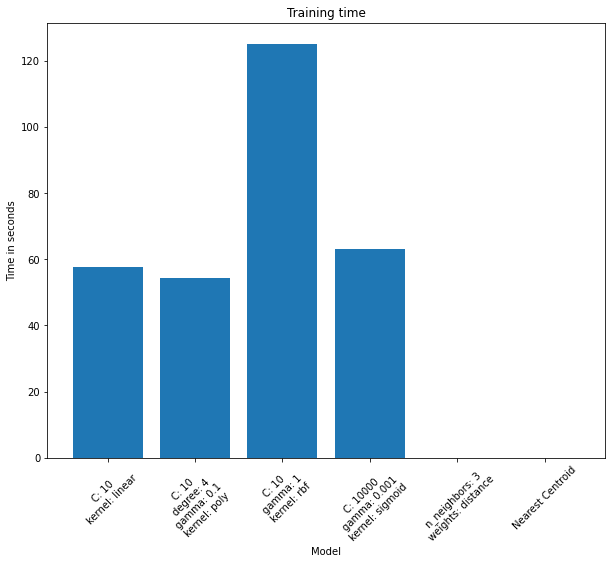
\includegraphics[width=0.6\linewidth]{figures/mnist/training_time.png}
    \caption{Χρόνος εκπαίδευσης για τη βάση MNIST}
    \label{fig:mnist_training_times}
\end{figure}

\subsubsection{Cifar-10}

Στο \autoref{fig:cifar_metrics} και στους \autoref{tab:cifar_train} και
\autoref{tab:cifar_test} φαίνονται τα αποτελέσματα των μετρικών για όλα τα
μοντέλα στο σύνολο εκπαίδευσης και ελέγχου για τις καλύτερες παραμέτρους στη
βάση Cifar-10.

Το μοντέλο του SVM με RBF πυρήνα έχει το καλύτερο αποτέλεσμα για όλες τις
μετρικές στο σύνολο ελέγχου όπως και στη βάση MNIST. Ακόμα, τα SVM μοντέλα έχουν
καλύτερα αποτελέσματα σε σχέση με τα μοντέλα των πλησιέστερων γειτόνων και του
πλησιέστερου κέντρου κλάσης.

Από το \autoref{fig:cifar_training_times} και τον \autoref{tab:cifar_train}
φαίνεται ο χρόνος εκπαίδευσης των μοντέλων. Το μοντέλο του SVM με πολυωνυμικό
πυρήνα έχει το μεγαλύτερο χρόνο εκτέλεσης. Επίσης, όπως και στη βάση MNIST τα
μοντέλα των πλησιέστερων γειτόνων και του πλησιέστερου κέντρου κλάσης έχουν πολύ
πιο μικρό χρόνο εκπαίδευσης σε σχέση με τα μοντέλα SVM.

\begin{table}[h]
\begin{tabular}{|l|c|c|c|c|c|}
\hline
\textbf{Model}                                                                     & \textbf{Accuracy} & \textbf{Precision} & \textbf{Recall} & \textbf{F1} & \textbf{Training Time (seconds)} \\ \hline
\begin{tabular}[c]{@{}l@{}}C: 1\\ kernel: linear\end{tabular}                      & 0,4189            & 0,416              & 0,4189          & 0,416       & 410,7339                         \\ \hline
\begin{tabular}[c]{@{}l@{}}C: 1\\ degree: 2\\ gamma: 1\\ kernel: poly\end{tabular} & 0,6943            & 0,6989             & 0,6943          & 0,695       & 823,6295                         \\ \hline
\begin{tabular}[c]{@{}l@{}}C: 10\\ gamma: 1\\ kernel: rbf\end{tabular}             & 0,9631            & 0,964              & 0,9631          & 0,9634      & 569,9598                         \\ \hline
\begin{tabular}[c]{@{}l@{}}C: 10000\\ gamma: 0.001\\ kernel: sigmoid\end{tabular}  & 0,4204            & 0,4175             & 0,4204          & 0,4175      & 603,1902                         \\ \hline
\begin{tabular}[c]{@{}l@{}}n\_neighbors: 1\\ weights: uniform\end{tabular}         & 1                 & 1                  & 1               & 1           & 0,0092                           \\ \hline
Nearest Centroid                                                                   & 0,3661            & 0,3626             & 0,3661          & 0,3575      & 0,0291                           \\ \hline
\end{tabular}
\centering
\caption{Μετρικές αποτελεσμάτων στο σύνολο εκπαίδευσης και χρόνος εκπαίδευσης
    για τη βάση Cifar-10.}
\label{tab:cifar_train}
\end{table}

\begin{table}[h]
\begin{tabular}{|l|c|c|c|c|c|}
\hline
\textbf{Model}                                                                     & \textbf{Accuracy} & \textbf{Precision} & \textbf{Recall} & \textbf{F1} \\ \hline
\begin{tabular}[c]{@{}l@{}}C: 1\\ kernel: linear\end{tabular}                      & 0,4092            & 0,4067             & 0,4092          & 0,4067      \\ \hline
\begin{tabular}[c]{@{}l@{}}C: 1\\ degree: 2\\ gamma: 1\\ kernel: poly\end{tabular} & 0,5463            & 0,5485             & 0,5463          & 0,5457      \\ \hline
\begin{tabular}[c]{@{}l@{}}C: 10\\ gamma: 1\\ kernel: rbf\end{tabular}             & 0,56              & 0,5626             & 0,56            & 0,5607      \\ \hline
\begin{tabular}[c]{@{}l@{}}C: 10000\\ gamma: 0.001\\ kernel: sigmoid\end{tabular}  & 0,4074            & 0,4046             & 0,4074          & 0,4048      \\ \hline
\begin{tabular}[c]{@{}l@{}}n\_neighbors: 1\\ weights: uniform\end{tabular}         & 0,3394            & 0,4238             & 0,3394          & 0,3307      \\ \hline
Nearest Centroid                                                                   & 0,369             & 0,3647             & 0,369           & 0,3601      \\ \hline
\end{tabular}
\centering
\caption{Μετρικές αποτελεσμάτων στο σύνολο ελέγχο για τη βάση Cifar-10.}
\label{tab:cifar_test}
\end{table}

\begin{figure}[H]
    \centering
    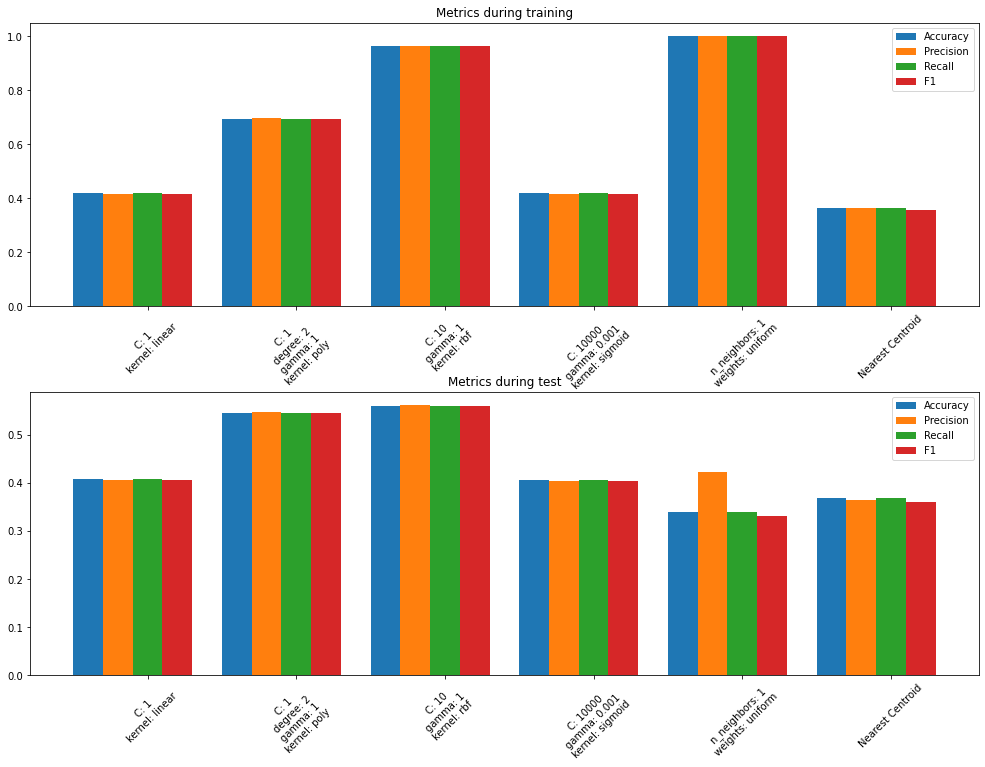
\includegraphics[width=\linewidth]{figures/cifar/all_metrics.png}
    \caption{Μετρικές για τη βάση Cifar-10}
    \label{fig:cifar_metrics}
\end{figure}

\begin{figure}[H]
    \centering
    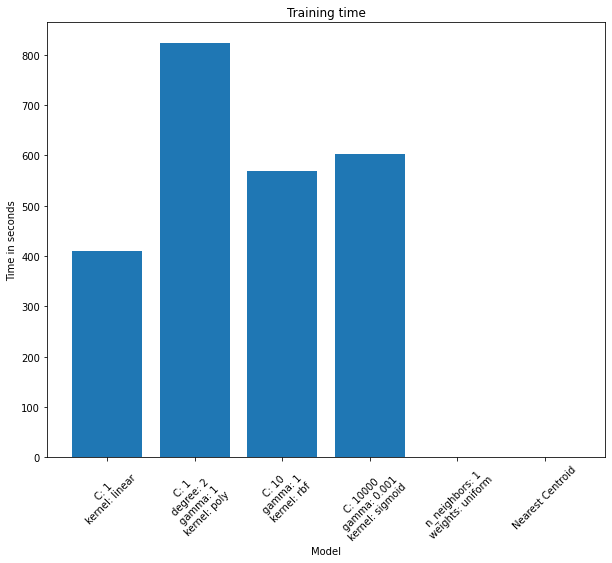
\includegraphics[width=0.6\linewidth]{figures/cifar/training_time.png}
    \caption{Χρόνος εκπαίδευσης για τη βάση Cifar-10}
    \label{fig:cifar_training_times}
\end{figure}

\subsection{Απόδοση καλύτερων μοντέλων}

\subsubsection{MNIST}

Το καλύτερο μοντέλο για τη βάση MNIST είναι το SVM με RBF πυρήνα. Στο
\autoref{fig:mnist_confusion} φαίνεται το confusion matrix γι᾽ αυτό το μοντέλο.
Από το σχήμα αυτό παρατηρείται ότι οι περισσότερες εσφαλμένες ταξινομήσεις
γίνονται όταν:

\begin{itemize}
    \item Η πραγματική κλάση είναι {\bf7} ενώ το μοντέλο την ταξινομεί στη
        {\bf2}.
    \item Η πραγματική κλάση είναι {\bf4} ενώ το μοντέλο την ταξινομεί στη
        {\bf9}.
    \item Η πραγματική κλάση είναι {\bf9} ενώ το μοντέλο την ταξινομεί στη
        {\bf4}.
    \item Η πραγματική κλάση είναι {\bf2} ενώ το μοντέλο την ταξινομεί στη
        {\bf8}.
\end{itemize}

Το μοντέλο αυτό "μπερδεύει" κλάσεις που έχουν παρόμοια μορφολογία όπως αυτή του
{\bf7} και του {\bf5} και του {\bf4} και του {\bf9}.

Από το \autoref{fig:mnist_wrong} φαίνονται μερικές από τις λάθος ταξινομήσεις
του μοντέλου. Από το σχήμα αυτό επιβεβαιώνεται η προηγούμενη παρατήρηση και
επίσης παρατηρείται ότι μερικές εικόνες δεν είναι τόσο εύκολο να ταξινομηθούν
και από έναν άνθρωπο.

\begin{figure}[H]
    \centering
    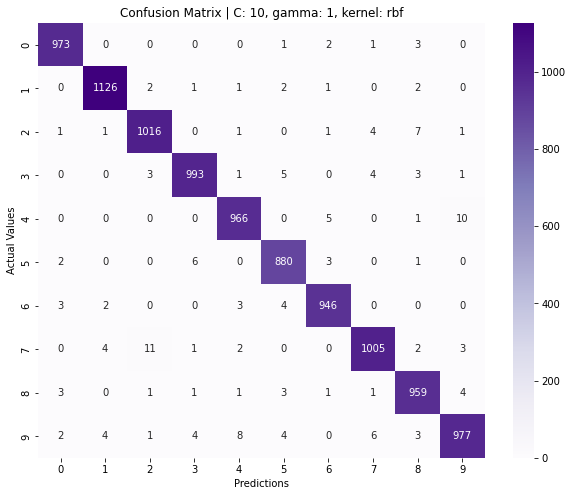
\includegraphics[width=0.6\linewidth]{figures/mnist/confusion_matrix.png}
    \caption{Confusion matrix για τη βάση MNIST}
    \label{fig:mnist_confusion}
\end{figure}

\begin{figure}[H]
    \centering

    \begin{subfigure}[t]{0.48\linewidth}
    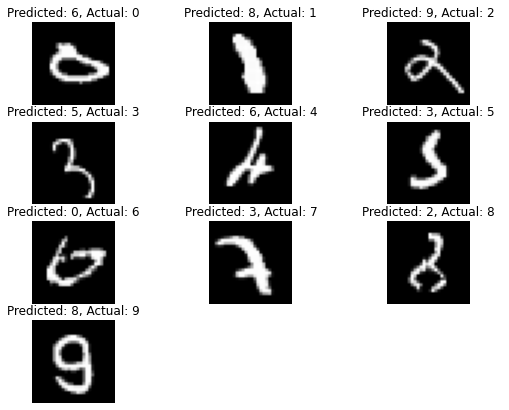
\includegraphics[width=\linewidth]{figures/mnist/wrong_results_1.png}
    \end{subfigure}
    \begin{subfigure}[t]{0.48\linewidth}
    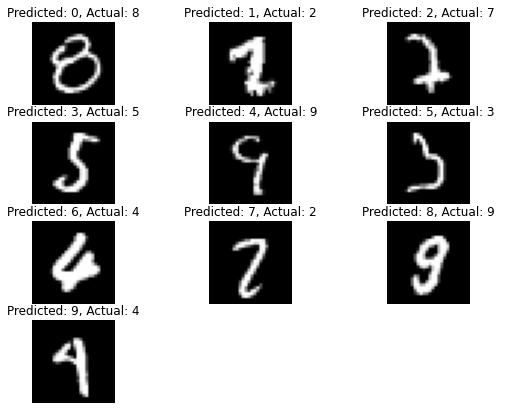
\includegraphics[width=\linewidth]{figures/mnist/wrong_results_2.png}
    \end{subfigure}

    \caption{Λάθος ταξινομήσεις του καλύτερου μοντέλου για τη βάση MNIST}
    \label{fig:mnist_wrong}
\end{figure}

\subsubsection{Cifar-10}

Το καλύτερο μοντέλο για τη βάση Cifar-10 είναι το SVM με RBF πυρήνα. Στο
\autoref{fig:cifar_confusion} φαίνεται το confusion matrix γι᾽ αυτό το μοντέλο.
Από το σχήμα αυτό παρατηρείται ότι οι περισσότερες εσφαλμένες ταξινομήσεις
γίνονται όταν:

\begin{itemize}
    \item Η πραγματική κλάση είναι {\bf σκύλος} ενώ το μοντέλο την ταξινομεί στη
        {\bf γάτα}.
    \item Η πραγματική κλάση είναι {\bf γάτα} ενώ το μοντέλο την ταξινομεί στη
        {\bf σκύλος}.
    \item Η πραγματική κλάση είναι {\bf ελάφι} ενώ το μοντέλο την ταξινομεί στη
        {\bf πουλί}.
    \item Η πραγματική κλάση είναι {\bf φορτηγό} ενώ το μοντέλο την ταξινομεί στη
        {\bf αυτοκινητιστικό} (automobile).
\end{itemize}

Παρατηρείται ότι το μοντέλο πραγματοποιεί λάθος ταξινομήσεις όταν οι κλάσεις
έχουν παρόμοια χαρακτηριστικά όπως π.χ. η κλάση του {\bf σκύλος} και της {\bf
γάτας} και του {\bf φορτηγού} και του {\bf αυτοκινητιστικό}. Επίσης λάθη
παρατηρούνται όταν το περιβάλλον της εικόνας μπορεί να είναι παρόμοιο όπως π.χ.
η κλάση του {\bf πλοίου} και του {\bf αεροπλάνου} (έχουν μπλε παρασκήνιο).
Τέλος, υπάρχουν λάθη που δεν είναι τόσο πολύ εξηγήσιμα όπως π.χ. η κλάση του
{\bf ελαφιού} και του {\bf πουλιού}.

Στο \autoref{fig:cifar_wrong} παρουσιάζονται μερικές λάθος ταξινομήσεις του
μοντέλου.

\begin{figure}[H]
    \centering
    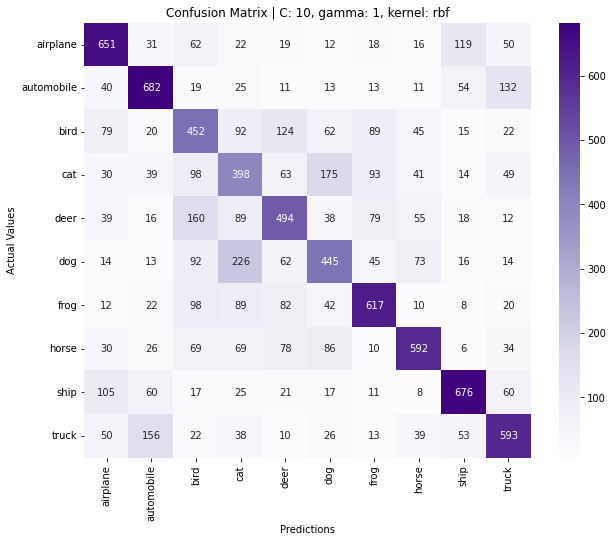
\includegraphics[width=0.6\linewidth]{figures/cifar/confusion_matrix.png}
    \caption{Confusion matrix για τη βάση Cifar-10}
    \label{fig:cifar_confusion}
\end{figure}

\begin{figure}[H]
    \centering

    \begin{subfigure}[t]{0.48\linewidth}
    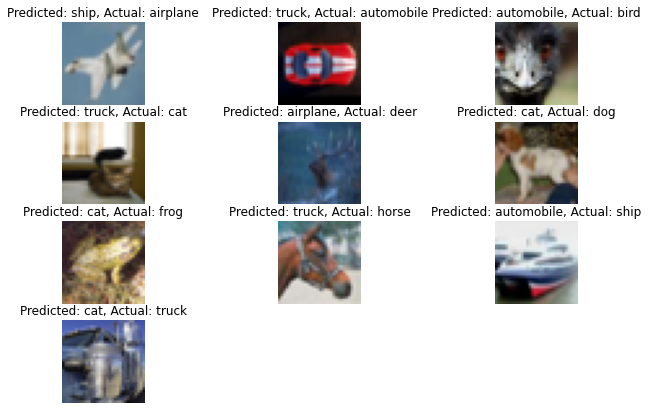
\includegraphics[width=\linewidth]{figures/cifar/wrong_results_1.png}
    \end{subfigure}
    \begin{subfigure}[t]{0.48\linewidth}
    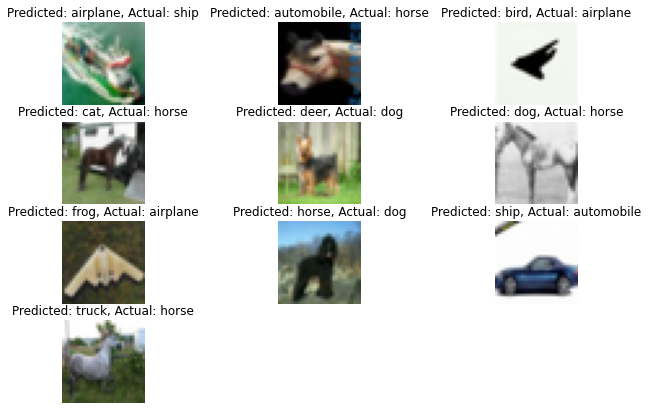
\includegraphics[width=\linewidth]{figures/cifar/wrong_results_2.png}
    \end{subfigure}

    \caption{Λάθος ταξινομήσεις του καλύτερου μοντέλου για τη βάση Cifar-10}
    \label{fig:cifar_wrong}
\end{figure}

\end{document}
